\chapter{Least Action, Euler--Lagrange, and Symmetry}

These notes follow Leonard Susskind's third lecture on classical mechanics. The lecture begins at the widest scale, with the claim that the laws of physics share a common form, and then narrows, step by step, to the variational argument that converts a global statement about an entire trajectory into a local differential equation. We keep the mathematical order of that argument intact. The retained board figures are drawn from Leonard Susskind's lecture, with visual curation by LazyingArt LLC and Video2Book, and they are used only where they genuinely witness notation, layout, or geometry on the board.

\section{The Common Form of Physical Law}

The lecture does not begin with a particle on a line. It begins with a larger claim: the laws of physics have a common form. Not every mathematical truth is a law of physics, and not every theorem of probability theory is a law of physics in the narrow sense that concerns us here. But the dynamical laws of classical physics, in all their different guises, can be cast into a single structural form. That form is the principle of least action.

This opening enlargement matters. We are not being told only that least action is a clever reformulation of Newtonian mechanics. We are being told that it is the common pattern in which a great deal of physics is written. Even thermodynamics, which is not ordinarily presented this way, is described as a statistical layer built on underlying microscopic laws that do have the form of a variational principle.

Only after this broad framing does the lecture turn to mechanics proper. And before the main derivation begins, Susskind pauses, characteristically, for two small pieces of mathematics that will do all the heavy lifting later on.

\section{Two Mathematical Tools Before the Main Derivation}

The first tool is integration by parts. The transcript is noisy in this portion of the lecture, but the mathematical move is clear and standard. We begin with the basic fact that the integral of a derivative over an interval is the difference of the function at the endpoints:
\begin{equation}
\int_{t_1}^{t_2}\dot F(t)\,dt = F(t_2)-F(t_1).
\end{equation}
Now take \(F(t)=f(t)g(t)\). The product rule gives
\begin{equation}
\frac{d}{dt}\big(fg\big)=\dot f\,g+f\,\dot g.
\end{equation}
Integrating this identity from \(t_1\) to \(t_2\), we obtain
\begin{equation}
\int_{t_1}^{t_2}\dot f\,g\,dt = [fg]_{t_1}^{t_2}-\int_{t_1}^{t_2}f\,\dot g\,dt.
\end{equation}
This is the form we will use later. It tells us that we may move the time derivative from one factor to the other, provided we pay for it with a minus sign and a boundary term.

\subsection{Question \& Answer}

\paragraph{Why is there a \(dt\) in the integral?}
The student interruption here is mathematically useful. Whenever we write an integral, we are integrating with respect to something. In this lecture the independent variable is time, so the integral must carry a \(dt\). The expression
\[
\int \dot f(t)
\]
is incomplete notation. What we mean is
\[
\int \dot f(t)\,dt.
\]
The question may sound elementary, but it forces the notation to become explicit, and in a variational derivation that explicitness matters.

The special case we shall need again and again is the case in which one factor vanishes at both endpoints. Then the boundary term disappears and the identity collapses to
\begin{equation}
\int_{t_1}^{t_2}\dot f\,g\,dt = -\int_{t_1}^{t_2}f\,\dot g\,dt.
\end{equation}
This is exactly the shape required later, when the variation of the path is fixed to vanish at the endpoints.

The second tool is even smaller, but conceptually crucial.

\begin{proposition}
If
\begin{equation}
\int_{t_1}^{t_2} a(t)f(t)\,dt = 0
\end{equation}
for every sufficiently arbitrary test function \(f(t)\), then \(a(t)=0\) throughout the interval.
\end{proposition}

\begin{proof}
The lecture's argument is the right one: choose \(f(t)\) to be concentrated in a tiny neighborhood of a point \(t_*\), and zero everywhere else. Then the integral isolates the value of \(a(t)\) near \(t_*\). If the integral must vanish for every such localized choice of \(f\), then \(a(t_*)\) must vanish. Since the point \(t_*\) was arbitrary, the function \(a(t)\) must vanish pointwise.
\end{proof}

This humble lemma is what allows us to turn an integral statement into a local differential equation. With these two tools in hand, we are ready for what Susskind calls the big one.

\section{Trajectories, Histories, and the Local--Global Tension}

A mechanical system is described by generalized coordinates
\[
q_1(t),\ q_2(t),\ \dots,\ q_n(t).
\]
To know the system's history is to know all of these functions of time. The lecture is very explicit on this point: what interests us is not merely a point in configuration space, but a whole trajectory, a whole history.

There are then two ways to formulate the laws of motion.

The local formulation tells us how to move forward from one point of the trajectory to a nearby one. Newton's law \(F=ma\) is the model example. If we know the coordinates and the velocities at one moment, then the differential law tells us how to continue the path.

The global formulation, by contrast, looks at the entire trajectory at once. It assigns to that trajectory a number called the action, and the true path is the one for which that action is minimized, or more precisely, stationary, among all nearby paths with the same endpoints.

The lecture then makes the bridge between these two points of view. If the true path minimizes the action globally between the initial and final times, it must also minimize the action locally between nearby points along the path. Otherwise we could improve that local piece and thereby improve the whole path. So a global least-action principle should imply a local differential equation. The rest of the lecture is the derivation of that equation.

\section{Varying the Path and Deriving the Euler--Lagrange Equation}

Let \(\hat q_i(t)\) denote the true trajectory. We deform it by adding a small multiple of an arbitrary function:
\begin{equation}
q_i(t)=\hat q_i(t)+\alpha f_i(t).
\end{equation}
The deformation functions are arbitrary except for one condition:
\begin{equation}
f_i(t_1)=f_i(t_2)=0.
\end{equation}
That condition keeps the endpoints nailed down. The varied path may wander in between, but it must still pass through the same initial and final points.

At this stage the lecture pauses naturally: we have spoken about minimizing the action, but we have not yet defined the action itself.

\begin{definition}
For a trajectory \(q_i(t)\) between \(t_1\) and \(t_2\), the action is
\begin{equation}
A[q]=\int_{t_1}^{t_2}L(q,\dot q,t)\,dt.
\end{equation}
For the mechanical examples in this lecture, the Lagrangian is
\begin{equation}
L=T-U,
\end{equation}
kinetic energy minus potential energy. But in the derivation itself we temporarily allow \(L\) to be any function of the coordinates, velocities, and possibly time.
\end{definition}

Because the varied path depends on \(\alpha\), the action becomes a function \(A(\alpha)\). The true trajectory corresponds to \(\alpha=0\). The lecture speaks of a minimum; the actual differential step uses the weaker statement that the action is stationary there:
\begin{equation}
\left.\frac{dA}{d\alpha}\right|_{\alpha=0}=0.
\end{equation}

Now differentiate the varied path with respect to \(\alpha\):
\begin{equation}
\frac{\partial q_i}{\partial \alpha}=f_i(t), \qquad
\frac{\partial \dot q_i}{\partial \alpha}=\dot f_i(t).
\end{equation}
Using the chain rule, the first variation of the action takes the standard form
\begin{equation}
\frac{dA}{d\alpha}
=
\int_{t_1}^{t_2}
\sum_i
\left(
\frac{\partial L}{\partial q_i}f_i
+
\frac{\partial L}{\partial \dot q_i}\dot f_i
\right)dt.
\end{equation}
The transcript is partially garbled at this point, but the move itself is unambiguous: the first term comes from varying \(q_i\), and the second comes from varying \(\dot q_i\).

We now use integration by parts on the term containing \(\dot f_i\). Since \(f_i(t_1)=f_i(t_2)=0\), the boundary term vanishes. Thus
\begin{equation}
\int_{t_1}^{t_2}
\frac{\partial L}{\partial \dot q_i}\dot f_i\,dt
=
-
\int_{t_1}^{t_2}
\frac{d}{dt}\left(\frac{\partial L}{\partial \dot q_i}\right)f_i\,dt.
\end{equation}
Substituting this back into the variation, we find
\begin{equation}
\frac{dA}{d\alpha}
=
\int_{t_1}^{t_2}
\sum_i
\left[
\frac{\partial L}{\partial q_i}
-
\frac{d}{dt}\left(\frac{\partial L}{\partial \dot q_i}\right)
\right]f_i\,dt.
\end{equation}
At \(\alpha=0\), stationarity requires this integral to vanish for every allowed set of functions \(f_i(t)\). By the arbitrary-function lemma, the bracket must vanish pointwise. Therefore
\begin{equation}
\frac{d}{dt}\left(\frac{\partial L}{\partial \dot q_i}\right)
=
\frac{\partial L}{\partial q_i}.
\end{equation}
This is the Euler--Lagrange equation. It is the precise form of the lecture's central claim: a global condition on the whole path has been converted into a local law at each instant along the path.

\begin{figure}
\centering

\includegraphics[width=0.72\textwidth]{lecture_03_figure_02.png}
\par
\begin{tikzpicture}
\draw[->] (0,0) -- (0,3.5) node[left] {$t$};
\draw[->] (0,0) -- (4.2,0) node[below] {$q$};
\fill (1.0,0.8) circle (1.4pt);
\fill (3.2,2.9) circle (1.4pt);
\draw (1.0,0.8) .. controls (1.5,1.5) and (2.3,2.2) .. (3.2,2.9);
\draw[dashed] (1.0,0.8) .. controls (1.7,1.1) and (2.5,2.6) .. (3.2,2.9);
\end{tikzpicture}
\caption{The board isolates the Euler--Lagrange time-derivative term while placing it beside a qualitative trajectory sketch. The redraw below keeps only the lecture's local idea: between fixed neighboring points, nearby paths may be compared.}
\end{figure}

\section{What the Euler--Lagrange Equation Says}

At this point the lecture turns from formal derivation to interpretation. It does so by naming the new objects that have appeared.

\begin{figure}
\centering

\includegraphics[width=0.62\textwidth]{lecture_03_figure_03.png}
\caption{The quantity obtained by differentiating the Lagrangian with respect to \(\dot q_i\) is introduced as canonical momentum.}
\end{figure}

We write
\begin{equation}
\pi_i=\frac{\partial L}{\partial \dot q_i}.
\end{equation}
This is the canonical momentum conjugate to the coordinate \(q_i\). The quantity
\begin{equation}
\frac{\partial L}{\partial q_i}
\end{equation}
is called the generalized force. In this language the Euler--Lagrange equation becomes
\begin{equation}
\frac{d\pi_i}{dt}=\frac{\partial L}{\partial q_i}.
\end{equation}
That already sounds more familiar: the time derivative of a momentum equals a force.

\subsection{Question \& Answer}

\paragraph{What does the Euler--Lagrange equation say in English?}
The lecture deliberately postpones this question until after the derivation, and then postpones it once more until examples are in view. The first answer is structural: the equation says that a global description of motion by least action is equivalent to a local description by differential equations.

The second answer is dynamical: once we identify \(\partial L/\partial \dot q_i\) as momentum and \(\partial L/\partial q_i\) as force, the equation begins to speak the language of \(F=ma\). The true path is the one whose action is stationary, and that global statement is exactly equivalent to a local force law along the path.

With that in mind, we now descend the lecture's staircase of examples.

\section{Worked Newtonian Examples and Translation Symmetry}

For one particle moving along a line,
\begin{equation}
L=\frac12 m\dot x^2-U(x).
\end{equation}
The coordinate \(q\) is here just \(x\). Then
\begin{equation}
\frac{\partial L}{\partial \dot x}=m\dot x,
\qquad
\frac{\partial L}{\partial x}=-\frac{dU}{dx}.
\end{equation}
Substituting into the Euler--Lagrange equation gives
\begin{equation}
m\ddot x=-\frac{dU}{dx}.
\end{equation}
So the formal variational equation reproduces Newton's equation of motion in the simplest case.

The lecture immediately inserts an important caution. If we had chosen \(L=T+U\), the sign of the force law would come out wrong. The Lagrangian is \(T-U\), not the energy. The conserved energy, when we derive it later, will be \(T+U\), not \(L\) itself.

For many Cartesian coordinates we simply repeat the same step coordinate by coordinate. If
\begin{equation}
T=\sum_{i=1}^{N}\frac12 m_i\dot x_i^2,
\qquad
L=T-U(x_1,\dots,x_N),
\end{equation}
then
\begin{equation}
p_i=\frac{\partial L}{\partial \dot x_i}=m_i\dot x_i,
\qquad
\frac{dp_i}{dt}=-\frac{\partial U}{\partial x_i}.
\end{equation}
This is just \(F=ma\) again, but now for each particle and each direction of space.

The next example is more revealing. Consider two particles on a line with coordinates \(x_1\) and \(x_2\), masses \(m_1\) and \(m_2\), and a translation-invariant interaction:
\begin{equation}
L=\frac12 m_1\dot x_1^2+\frac12 m_2\dot x_2^2-U(x_1-x_2).
\end{equation}
Translation invariance means that the potential depends only on the separation, not on the absolute position of the pair.

\begin{figure}
\centering
\begin{tikzpicture}
\draw[thick] (-3.0,0) -- (3.0,0);
\fill (-1.6,0) circle (1.6pt);
\fill (1.0,0) circle (1.6pt);
\draw (-1.6,0.35) node {$m_1$};
\draw (1.0,0.35) node {$m_2$};
\draw (-1.6,-0.35) node {$x_1$};
\draw (1.0,-0.35) node {$x_2$};
\draw[->] (-2.2,1.0) -- (-0.9,1.0) node[midway,above] {$a$};
\draw[->] (0.4,1.0) -- (1.7,1.0);
\end{tikzpicture}
\caption{A rigid translation by the same amount \(a\) moves both particles but leaves the separation \(x_1-x_2\) unchanged.}
\end{figure}

To make the chain rule explicit, set
\[
d=x_1-x_2.
\]
Then \(U=U(d)\), and
\begin{align}
\frac{\partial U}{\partial x_1}
&=
\frac{dU}{dd}\frac{\partial d}{\partial x_1}
=
\frac{dU}{dd},\\
\frac{\partial U}{\partial x_2}
&=
\frac{dU}{dd}\frac{\partial d}{\partial x_2}
=
-\frac{dU}{dd}.
\end{align}
Therefore
\begin{equation}
\frac{\partial U}{\partial x_2}=-\frac{\partial U}{\partial x_1}.
\end{equation}
The two Euler--Lagrange equations are
\begin{equation}
\frac{dp_1}{dt}=-\frac{\partial U}{\partial x_1},
\qquad
\frac{dp_2}{dt}=-\frac{\partial U}{\partial x_2}.
\end{equation}
Adding them gives
\begin{equation}
\frac{d}{dt}(p_1+p_2)=0.
\end{equation}
So total linear momentum is conserved.

This is the lecture's first clean example of a much larger pattern. Because the action is invariant under a continuous translation, there is an associated conservation law. Here the symmetry is translation invariance, and the conservation law is conservation of linear momentum.

The lecture briefly notes another possibility. If we strengthened the potential to a function of \(|x_1-x_2|\), there would also be an inversion symmetry. But that is a discrete symmetry. The conservation law on display here comes from the continuous symmetry.

\section{Two Coordinates, One Broken Symmetry, and Rotational Invariance}

We now move to a particle near the surface of the Earth, described by two coordinates \(x\) and \(y\), with \(x\) horizontal and \(y\) vertical. The stable board evidence is the kinetic term, and the transcript supplies the potential:
\begin{equation}
T=\frac12 m\dot x^2+\frac12 m\dot y^2,
\qquad
U=mgy.
\end{equation}
Hence
\begin{equation}
L=\frac12 m\dot x^2+\frac12 m\dot y^2-mgy.
\end{equation}

\begin{figure}
\centering

\includegraphics[width=0.78\textwidth]{lecture_03_figure_04.png}
\par
\begin{tikzpicture}
\draw[->] (0,0) -- (4.2,0) node[below] {$x$};
\draw[->] (0,0) -- (0,3.0) node[left] {$y$};
\draw[thick] (-0.6,0) -- (4.2,0);
\fill (2.3,1.8) circle (1.6pt);
\draw (2.5,1.95) node[right] {$m$};
\end{tikzpicture}
\caption{The lecture frame gives the two-coordinate kinetic term and the simple near-Earth setup. The redraw regularizes only the stable geometry: horizontal \(x\), vertical \(y\), and a particle above the surface.}
\end{figure}

Because \(L\) does not depend explicitly on \(x\), the \(x\)-equation reads
\begin{equation}
\frac{d}{dt}(m\dot x)=0.
\end{equation}
So the horizontal component of momentum is conserved. But the \(y\)-equation is different:
\begin{equation}
\frac{d}{dt}(m\dot y)=-mg.
\end{equation}
There is no conservation of vertical momentum. That is exactly what the lecture wants us to notice: one symmetry survives, the other does not.

The side discussion about shifting \(y\) is worth keeping in its cleaned mathematical form. We may add a constant to the potential without changing the physics, since derivatives of \(U\) are unchanged. But that is not the same as translating the coordinate \(y\). A true \(y\)-translation changes \(U=mgy\), so the Lagrangian is not invariant under vertical shifts. Accordingly there is no conserved \(y\)-momentum.

The lecture now makes a broader claim. The principle of least action does not depend on the coordinates we use. Rectangular coordinates, polar coordinates, or some more exotic system may make the formulas look simpler or more complicated, but the underlying action principle is the same.

So let us pass to polar coordinates for a particle moving in a plane. The coordinates are \(r\) and \(\theta\), and the history is now given by the pair \(r(t)\), \(\theta(t)\). The lecture derives the kinetic energy geometrically by decomposing the velocity into radial and perpendicular components:
\begin{equation}
v_r=\dot r,
\qquad
v_\perp=r\dot\theta.
\end{equation}
Therefore
\begin{equation}
T=\frac12 m\left(\dot r^2+r^2\dot\theta^2\right).
\end{equation}

\begin{figure}
\centering
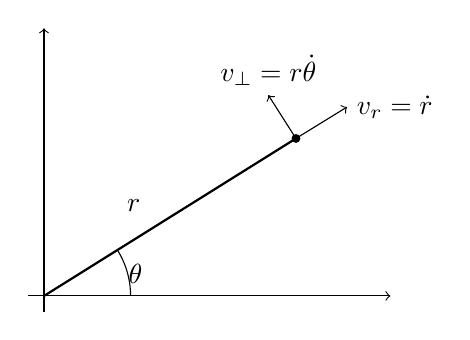
\begin{tikzpicture}
\draw[->] (-0.2,0) -- (4.4,0);
\draw[->] (0,-0.2) -- (0,3.4);
\draw[thick] (0,0) -- (3.2,2.0);
\fill (3.2,2.0) circle (1.6pt);
\draw (1.35,0.95) node[above left] {$r$};
\draw (1.1,0) arc (0:32:1.1);
\draw (0.95,0.28) node[right] {$\theta$};
\draw[->] (3.2,2.0) -- (3.85,2.4) node[right] {$v_r=\dot r$};
\draw[->] (3.2,2.0) -- (2.85,2.55) node[above] {$v_\perp=r\dot\theta$};
\end{tikzpicture}
\caption{Polar-coordinate geometry reconstructed from the lecture argument. The velocity splits into a radial piece \(\dot r\) and a perpendicular piece \(r\dot\theta\).}
\end{figure}

Now take a central potential,
\begin{equation}
U=U(r),
\end{equation}
so that the Lagrangian is
\begin{equation}
L=\frac12 m\left(\dot r^2+r^2\dot\theta^2\right)-U(r).
\end{equation}
The key point is not the full radial equation. The key point is that \(L\) does not depend explicitly on \(\theta\). Therefore \(\theta\) is a cyclic coordinate, and
\begin{equation}
\frac{\partial L}{\partial \dot\theta}=mr^2\dot\theta
\end{equation}
is conserved:
\begin{equation}
\frac{d}{dt}\left(mr^2\dot\theta\right)=0.
\end{equation}
So
\begin{equation}
mr^2\dot\theta=\mathrm{const}.
\end{equation}
This is conservation of angular momentum. It immediately explains the ice-skater effect mentioned in the lecture: if \(r\) decreases, then \(\dot\theta\) must increase so that the product \(mr^2\dot\theta\) remains fixed.

Once again the conserved quantity comes from a symmetry. Here the symmetry is rotational invariance. The pattern is now fully visible:
\[
\text{translation invariance} \longrightarrow \text{linear momentum conservation},
\qquad
\text{rotational invariance} \longrightarrow \text{angular momentum conservation}.
\]

\section{Summary}

The lecture begins with a broad declaration and ends with a pattern. The broad declaration is that least action is the common form of physical law. The derivation in the middle shows how a global variational statement becomes the local Euler--Lagrange equation,
\[
\frac{d}{dt}\left(\frac{\partial L}{\partial \dot q_i}\right)=\frac{\partial L}{\partial q_i}.
\]
The examples then translate that formal result back into familiar language: for ordinary mechanical systems it reproduces \(F=ma\), and when a coordinate does not appear explicitly in the Lagrangian, the conjugate momentum is conserved.

By the end of the lecture, the main lesson is no longer only the equation itself. It is the relationship between symmetry and conservation law. Translation symmetry yields linear momentum conservation. Rotational symmetry yields angular momentum conservation. The action principle is the framework in which both statements become transparent.